\chapter{Adaboost per classificazione binaria}
\vspace{1cm}
Adaboost, diminutivo di Adaptive Boosting, \`e uno tra gli algoritmi di Data Mining pi\`u utilizzati. 
Fu proposto da Yoav Freund e Robert Schapire, i quali hanno vinto il prestigioso ``Godel Prize'' (premio assegnato ai migliori lavori in
computer science) nel 2003 per il loro lavoro.\\
\`E molto accurato, semplice e con diverse applicazioni possibili, risulta meno suscettibile al rischio di overfitting rispetto ad altri 
algoritmi di apprendimento; pu\`o, inoltre, essere utilizzato insieme ad altri tipi di algoritmi di apprendimento per migliorare le prestazioni di questi algoritmi.
I difetti che presenta questo filtro includono il fatto che risulta sensibile agli outliers e ad i ``noisy'' data, ovvero ai dati sporchi.
Si basa sull'idea di creare una regola di predizione altamente accurata combinandone diverse dette ``deboli''. Risulta empiricamente che Adaboost riduce significativamente
l'errore di qualsiasi classificatore debole.\\
\newline

Si denota con {\begin{math}X\end{math}} lo spazio delle istanze mentre 
con {\begin{math}Y \end{math}} quello delle possibili etichette (ovvero i possibili modi in cui l'istanza viene classificata).
Si assume \begin{math}Y =\left\{-1,+1\right\}\end{math}. Dato un weak learner (``classificatore debole'') e un training set {\begin{math}D = (x_1,y_1),(x_2,y_2),..,(x_m,y_m)\end{math}}, 
dove {\begin{math} x_i \in X \end{math}} e {\begin{math} y_i \in Y \end{math}} (i=1,..,m), l'algoritmo Adaboost funziona come segue.\\
\newline
Inizialmente assegna pesi uguali a tutti gli esempi di training {\begin{math} (x_i,y_i)\end{math}} con (i=1,..,m).
Si denota come {\begin{math} D_t \end{math}}, la distribuzione dei pesi al t-esimo passo di apprendimento.

\newpage
\vspace{1.5cm}


Dal training set D e dalla 
distribuzione dei pesi
 {\begin{math} D_t \end{math}}, l'algoritmo genera 
 un weak learner {\begin{math} h_t:X \to Y \end{math}}, richiamando il weak learner
di partenza. Successivamente usa gli esempi di training per testare {\begin{math} h_t \end{math}} e i pesi degli esempi classificati in modo scorretto vengono
incrementati. Quindi, si ottiene una distribuzione dei pesi aggiornata, {\begin{math} D_{t+1} \end{math}}.\\
 Dal training set e da {\begin{math} D_{t+1} \end{math}},
Adaboost genera un altro classificatore debole richiamando nuovamente il weak learner di partenza. Il processo \`e cos\`i ripetuto per T volte. 
Il modello finale \`e la combinazione lineare dei T weak learners in base ai pesi determinati durante il processo di training.\\
\newline

Di seguito si riporta uno schema delle varie fasi:\\
\newline
\begin{itemize}
\item Sia {\begin{math}D = (x_1,y_1),(x_2,y_2),..,(x_m,y_m)\end{math}}
\item Si inizializza il vettore dei pesi: \begin{math} D_1(i)=1/m \end{math}
\item Il processo viene effettuato per T iterazioni 
\item Sia \begin{math} \mathcal{L} \end{math} weak learner iniziale una funzione di due variabili  \begin{math}(D,D_t)\end{math} a valori in {\begin{math}Y \end{math}}
\end{itemize}

\begin{enumerate}

 \item  \begin{math} h_t=\mathcal{L}(D,D_t)\end{math} viene fatto il train di un weak learner  \begin{math} h_t\end{math} da D usando la distribuzione
\begin{math} D_t\end{math}
\item \begin{math} \varepsilon_t=Pr{_i\sim D_i} [h_t(x_i\ne y_i)] \end{math}   misura l'errore di \begin{math} h_t\end{math}
\item \begin{math} \alpha_t=\frac{1}{2}\ln\frac{1-\varepsilon_t}{\varepsilon_t}  \end{math} 
determina il peso di \begin{math} h_t\end{math}

\item \begin{math} D_{t+1}(i)=\frac{D_t(i)}{Z_t}\times \begin{cases} exp(-\alpha_t) & se h_t(x_i)=y_i \\
                                                         exp(\alpha_t) & se h_t(x_i)\ne y_i
                                                       
                                                      \end{cases} =\frac{D_t(i)exp(-\alpha_ty_ih_t(x_i))}{Z_t} \end{math} \\
\newline
Aggiorna la distribuzione, dove \begin{math}Z_t \end{math} \`e un fattore di normalizzazione che permette a \begin{math}D_{t+1} \end{math}
di essere una distribuzione.


\end{enumerate}
L'output sar\`a:
\begin{center}
 \begin{math} H(x)=sign(\sum_{t=1}^T \alpha_t h_t(x)) \end{math}
\end{center}

\newpage
\vspace{1.5cm}

Viene riportato un breve esempio di applicazione dell'algoritmo:
abbiamo a disposizione un dataset di 10 elementi, appartenenti a due classi differenti, e 3 classificatori deboli.


\begin{figure}[!h]
\centering
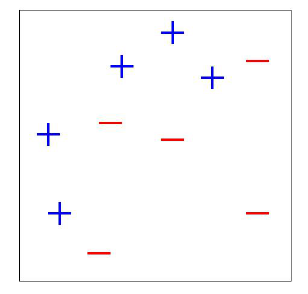
\includegraphics[width=0.6\textwidth]{esempio_adaboost1.png}%
 \caption{\textit{Disposizione dei dati.}}
 \label{grafico1}
\end{figure}
Inizialmente entrambe le popolazioni hanno lo stesso peso. La ``frontiera'' tra le due popolazioni \`e evidente ma non \`e lineare.
\begin{figure}[!h]
\centering
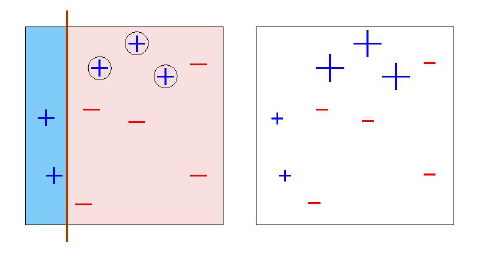
\includegraphics[width=0.8\textwidth]{esempio_adaboost2.png}%
 \caption{\textit{Esito del primo classificatore e conseguente aggiornamento dei pesi.}}
 \label{grafico2}
\end{figure}
\newpage
Individuato il ``primo'' classificatore, possiamo notare come classifica correttamente la classe ``-'', ma commette 3 errori, tali osservazioni verranno
pesate maggiormente al passo successivo. Dalle formule per il calcolo dei coefficienti, 
otteniamo \begin{math}\alpha_1=0.42\end{math}.


\begin{figure}[!h]
\centering
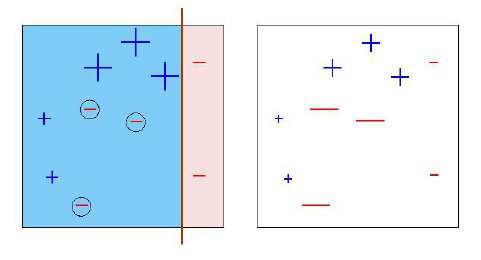
\includegraphics[width=0.8\textwidth]{esempio_adaboost3.png}%
 \caption{\textit{Esito del secondo classificatore e conseguente aggiornamento dei pesi.}}
 \label{grafico3}
\end{figure}

I risultati del secondo classificatore sono analoghi a quelli del primo, \`e di grande importanza, per\`o, notare come variano i pesi delle osservazioni.
Il valore del coefficiente di tale classificatore \`e \begin{math}\alpha_2=0.66\end{math}.
\begin{figure}[!h]
\centering
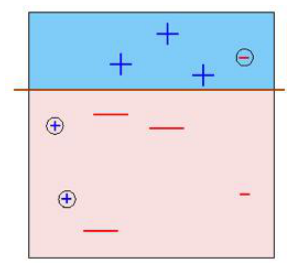
\includegraphics[width=0.6\textwidth]{esempio_adaboost4.png}%
 \caption{\textit{Esito del terzo classificatore.}}
 \label{grafico4}
\end{figure}
\newpage
Introduciamo il terzo classificatore. Questo commette 3 errori, ma i loro pesi sono nettamente inferiori rispetto agli altri,
perch\`e tali osservazioni avevano gi\`a ottenuto un esito corretto dai precedenti classificatori, otteniamo cos\`i un valore per
il coefficiente \begin{math}\alpha_3=0.91\end{math}. Osserviamo i risultati cos\`i ottenuti:


\begin{figure}[!h]
\centering
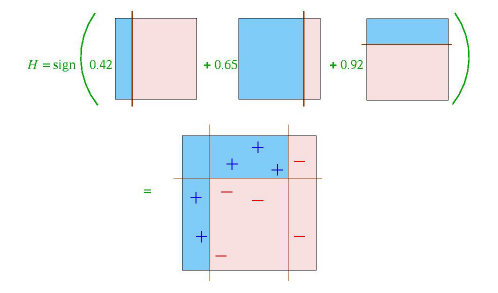
\includegraphics[width=0.9\textwidth]{esempio_adaboost5.png}%
 \caption{\textit{Esito del classificatore finale.}}
 \label{grafico5}
\end{figure}





